\documentclass[10pt, conference, compsocconf]{IEEEtran}
% Add the compsocconf option for Computer Society conferences.
%
% If IEEEtran.cls has not been installed into the LaTeX system files,
% manually specify the path to it like:
% \documentclass[conference]{../sty/IEEEtran}
\usepackage{cite}

\usepackage[cmex10]{amsmath}
\usepackage{amssymb}

\usepackage{algorithm}
\usepackage{array}
\usepackage{algpseudocode}
\usepackage{indentfirst}

\ifx\pdfoutput\undefined
\usepackage{graphicx}
\else
\usepackage[pdftex]{graphicx}
\fi
\usepackage{epstopdf}

%\usepackage[pdftex]{graphicx}
\usepackage[tight,footnotesize]{subfigure}
\usepackage{multirow}


%\usepackage{algorithmic}


\begin{document}

\title{Evaluation of Design Trade-offs for Adders\\ in Approximate Datapath}
%Evaluation of Design Trade-offs for Approximate Arithmetic Operators
%Evaluation of Optimum Arithmetic Operators For Approximate Datapath Design

\author{\IEEEauthorblockN{Kan Shi and George A. Constantinides}
\IEEEauthorblockA{Department of Electrical and Electronic Engineering\\
Imperial College London\\
London, UK\\
Email: \{k.shi11, g.contantinides\}@imperial.ac.uk}
\vspace{1ex}
%\and
%\IEEEauthorblockN{Authors Name/s per 2nd Affiliation (Author)}
%\IEEEauthorblockA{line 1 (of Affiliation): dept. name of organization\\
%line 2: name of organization, acronyms acceptable\\
%line 3: City, Country\\
%line 4: Email: name@xyz.com}
}


\maketitle


\begin{abstract}
Releasing the stringent accuracy requirement would potentially offer greater freedom to create a design with better performance or energy efficiency. In this paper, we evaluate the design trade-offs for adders, which are key building blocks for many applications. We demonstrate the optimum design metric for adders, under the consideration of various design constraints, such as accuracy, operating frequency, silicon area, different types of adder structure and alternative form of computer arithmetic for adder implementation. Two design scenarios are compared: one is the conventional design scenario where timing closure is met by adjusting operand word-lengths. The other is an overclocking scenario where timing violations are allowed to occur. We show that applying the overclocking approach to ripple carry adders can be more beneficial than using fast adders to achieve similar latency, because the worst cases only happen with very small probabilities. We also show that using the conventional approach on adders with new form of computer arithmetic is optimal for a wide range of design constraints.

%We show that instead of losing precision to ensure timing closure, allowing timing violations to happen can be beneficial, because the worst case scenario only happens with a very small probability.


\end{abstract}

\begin{IEEEkeywords}
approximate computing; adder; overclocking; online arithmetic;

\end{IEEEkeywords}


\section{Introduction}
Circuit performance has increased tremendously over the past decades. However, in recent years people have observed an end of performance scaling~\cite{DarkSilicon2011} due to the improvement of CMOS technology to the nanometer regime. In order to boost circuit performance, two standard design techniques are commonly adopted: one is to heavily pipeline the datapath, the other is to reduce the design precision. For the first technique, pipelining can be used to increase operating frequency, whereas the overall computational latency will not be affected. Therefore the utilization of this technique is limited in many embedded applications, which are often designed with strict latency specifications. The second technique is common especially with FPGA technology, which embodies the flexibility to implement customized variable representation and is able to optimize the operand word-length across the entire datapath to meet a given performance and area constraint~\cite{GeorgeDT11}. However, the precision loss will inevitably introduce quantization errors into the design.

Unfortunately, in both situations circuits are designed for the worst cases. In order to avoid potential timing violations, timing analysis tools tend to provide a conservative critical path delay by adding guard bands and timing margins. However, continuing with this approach will become increasingly expensive and difficult as technology shrinks.

To tackle this problem, a large volume of research activities were focused on the design methodology of relaxing the $100\%$ accuracy requirements and design constraints, while reasoning about the corresponding benefits and costs. Studies have shown that computing approximately provides extra opportunities to design circuits with better performance and less energy consumption. A brief review of the work in this area is given in Section~\ref{sec:Background}.

In this paper, we provide detailed evaluations of design trade-offs for adders, which are key arithmetic primitives for a broad range of applications. In order to provide the optimum design choice for adders, we examine several design constrains and options, such as accuracy, operating frequency, silicon area, different types of adder structure, as well as different forms of computer arithmetic for adder implementation. In comparison to the conventional design scenario that timing closure is achieved by truncating the operand word-length, we take a radical step forward by adopting an alternative design scenario, which is named ``overclocking scenario''. In this case, circuits are operated far beyond the conservation region with full precision, while timing violation can be tolerated. Previous work has shown that for many applications, it is preferable to follow the overclocking scenario because the worst case is triggered only by certain input patterns and hence it happens rarely~\cite{SKfccm13}. In addition to the adder structures that are created based on standard binary arithmetic, such as ripple carry adder and carry select adder, we also evaluate adder with ``online arithmetic''~\cite{Ercegovac_OnlineOverview}, which employs different style of data representation to eliminate carry propagation. We demonstrate experimentally on FPGAs that for limited area budgets, applying the overclocking approach to ripple carry adders can be more beneficial than using fast adders to achieve similar latency. With more relaxed area constraints, the online adder outperforms in terms of accuracy or performance. Potentially our study will provide circuit designers with guidance and extra options when balancing between various design trade-offs.

In summary, the main contributions of this paper are:
\begin{enumerate}
  \item Detailed evaluation of three adder structures: ripple carry adder, carry select adder and online adder;
  \item Comparison of design scenarios and demonstration of the optimum design choice under the consideration of trade-offs between accuracy, performance and area.
\end{enumerate}

The rest of this paper is organized as follows: we first provide a brief overview of the relevant work in this area, together with the background knowledge of online arithmetic in Section~\ref{sec:Background}. The comparison between different adder structures and design trade-offs are detailed in Section~\ref{sec:diff_adder}. This is followed by the evaluation of optimum design choices when considering trade-offs between accuracy, performance and area in Section~\ref{sec:optimum_adder}. The conclusion and suggestions of possible future work is given in Section~\ref{sec:conclusion}.


\section{Background}\label{sec:Background}
\subsection{Approximate Datapath Design}
The International Technology Roadmap for Semiconductors (ITRS) has identified that additional benefits of manufacturing, test, power and timing can be achieved by releasing the requirement of absolute correctness~\cite{semiconductor2007international}. This fact has inspired a series of studies to create circuits operating beyond the worst cases and the safety margins. Typically this can be achieved by either reducing the supply voltage~\cite{NonUniformScaling} or increasing the operating frequency beyond the rated value~\cite{SKfccm13,JoshFCCM2012}. The Razor project~\cite{Razor2004} served as one of the exemplary designs, in which both supply voltage and clock frequency were scaled over the most conservative value, while the error rate was monitored by using a self-checking circuit. It was shown that over $30\%$ power saving can be obtained at the cost of around $1\%$ errors.

Another stream of research was focusing on proposing either approximate circuit structures or design tools to trade accuracy for performance and/or energy benefits. Work in this area was inspired by the fact that many applications, e.g. image processing and machine learning, were naturally error resilient. For example, code analysis tools~\cite{Truffle2012Uwash,EnerJ2011Uwash} were developed to divide a program into precise parts and approximate parts, which can then be mapped to hardware components with different speed-grades and supply voltages. As for the approximate hardware, numerous forms of architectures were designed for basic arithmetic operators such as adders~\cite{ApproximateAdderTC} and multipliers~\cite{ApproximateMultDATE}. For example, a under-designed multiplier unit was proposed, of which the worst case was replaced by a normal case based on straightforward Karnaugh-Map analysis~\cite{Undersigned2x2multiplier}. However, many of these techniques are designed at gate-level or transistor-level, and they cannot be directly applied onto existing hardware platforms such as FPGAs.

In this paper, we overcome the previous limitations by comparing two standard adder structures: ripple carry adder and carry select adder, which are widely employed in mainstream hardware platforms. We also compare a type of adder with ``online arithmetic'', which can be also found when designing fast multipliers and embedded processors~\cite{RedundantMult_1987}. It is argued that our approach can be efficiently applied to existing designs, and we back up this hypothesis based on FPGA experiments.



\subsection{Online Arithmetic}

As an alternative form of computer arithmetic, online arithmetic has been used in numerous applications such as signal processing and control algorithms~\cite{Online_FPGADSP,Online_Control}. Online arithmetic was originally designed for digit-serial operation, as illustrated in Fig~\ref{Fig:OnlineDataFlow}. It can be seen that in order to generate the first output digit, $\delta$ digits of inputs are required, where $\delta$ is called the ``online delay''. $\delta$ is normally a small constant, which is independent of the precision. For ease of discussion, for the rest of this paper, the input data is assumed to be fixed point numbers in the range $(-1,1)$. Based on this premise, the online representation of $N$-digit operands and result at iteration $j$ are given by (\ref{Eq:Online_Operands}), where $j\in[-\delta,N-1]$ and $r$ denotes the radix \cite{Ercegovac_Book}.
%
\begin{figure}[tbp]
  \centering
  %\vspace{-2.5ex}
  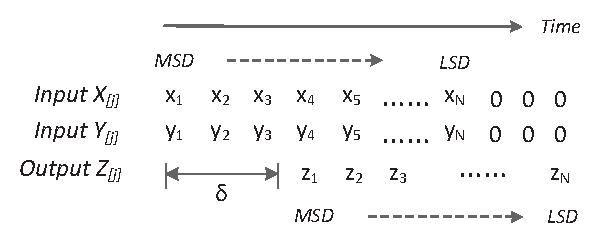
\includegraphics[width=.42\textwidth]{./figures/OnlineArithmetic_DataFlow.eps}
  %\vspace{-1ex}
  \caption{Dataflow in digit-serial online arithmetic, in which both inputs and outputs are processed from the MSD to the LSD. $\delta$ denotes the online delay.}
  %\vspace{-2ex}
  \label{Fig:OnlineDataFlow}
\end{figure}
%
\begin{eqnarray}\label{Eq:Online_Operands}
\footnotesize
  X_{[j]}=\sum_{i=1}^{j+\delta}x_ir^{-i},~Y_{[j]}=\sum_{i=1}^{j+\delta}y_ir^{-i},~Z_{[j]}=\sum_{i=1}^{j}z_ir^{-i}
\normalsize
\end{eqnarray}

MSD-first operation is possible only if a redundant number system is used. Normally there are two most commonly used redundant number representations: carry-save (CS) \cite{CSadder} and signed-digit (SD) \cite{RedundantNumber}. With SD representation, each digit is represented using a redundant digit set $\{-a, \cdots,-1,0, 1, \cdots, a\}$, where $a\in[r/2,r-1]$. In comparison, the standard non-redundant representation only uses a digit set $\{0,\cdots,r-1\}$. Thus a standard number corresponds to several possible redundant representations. For example, the binary number $0.011$ can be represented in SD form as $0.1\overline{1}1$, $0.10\overline{1}$ or $0.011$ among many other possible representations.

Due to the redundancy, the MSDs of the result can be calculated using partial information from both inputs. Then the value of the number can be revised using the subsequent digits, because each number has multiple representations.

\section{Design Trade-offs of Different Adder Structures}\label{sec:diff_adder}
\subsection{Ripple Carry Adder}\label{subsec:rca}
Adders serve as a key building block for arithmetic operations. In general, the ripple carry adder (RCA) is the most straightforward and widely used adder structure. As such, in our previous work we proposed probabilistic models of overclocking errors for RCA~\cite{SKfccm13}. A brief summary of the models is described below.
%
\begin{figure}[tbp]
  \centering
  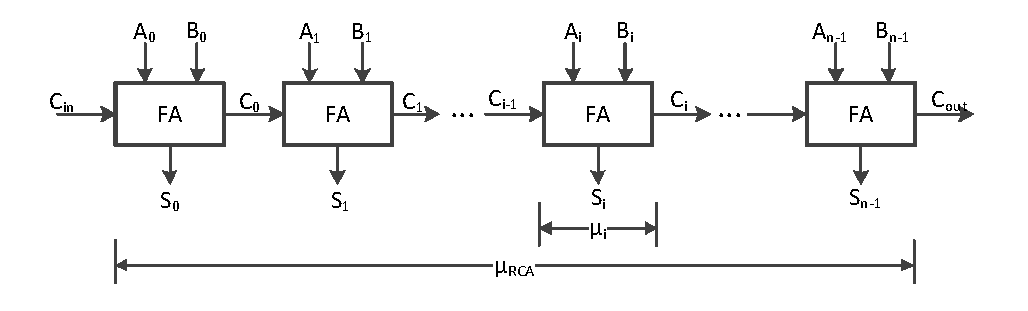
\includegraphics[width=.5\textwidth]{./figures/RCA.pdf}
  \vspace{-4ex}
  \caption{An $n$-bit ripple carry adder. $\mu_i$ and $\mu_{RCA}$ denote the propagation delay of a full adder and the overall delay of RCA, respectively.}
  \vspace{-2ex}
  \label{Fig:rca}
\end{figure}

For an $n$-bit RCA, it is composed of $n$ serial-connected full adders (FA) as shown in Fig.~\ref{Fig:rca}. Typically the maximum frequency of RCA is determined by the longest carry propagation. Under the assumption that the carry propagation delay of each FA is a constant value $\mu_i=\mu$, the critical path of the RCA is: $\mu_{RCA}=n\mu$. For the sampling period $T_S$, it follows that if $T_S\geqslant\mu_{RCA}$, correct result will always be sampled. Otherwise, intermediate result will be sampled and potentially generating overclocking errors. The mean value of overclocking error is modeled~\cite{SKfccm13} as given by (\ref{Eq:MeanError_RCA}), where coefficient $b$ is given in (\ref{Eq:b}) and it determines the maximum length of error-free carry propagation.
%
\begin{eqnarray}\label{Eq:MeanError_RCA}
    E_{oc}=\left\{
        \begin{matrix}
            2^{-b}-2^{-n-1}, & \textrm{if $b\leq n$}\\
            0, & \textrm{otherwise}
        \end{matrix}
        \right.
\end{eqnarray}
\vspace{-1.5ex}
%
\begin{eqnarray}\label{Eq:b}
    b:=\left\lceil \frac{T_S}{\mu} \right\rceil=\left\lceil \frac{1}{\mu\cdot f_S}\right\rceil
\end{eqnarray}
\vspace{-1ex}
\normalsize

In the conventional scenario, a specific timing target can be met by truncating the word-length of RCA while timing violation is not permitted. This will result in truncation error for most data.  The mean value of truncation error is also modeled~\cite{SKfccm13} as given by~(\ref{Eq:MeanTruncError_RCA}), where parameters $k$ and $n$ denote the word-length of RCA before and after truncation, respectively.
%
\begin{eqnarray}\label{Eq:MeanTruncError_RCA}
    E_{trad}=\left\{
        \begin{matrix}
            2^{-n}-2^{-k}, & \textrm{if $n<k$}\\
            0, & \textrm{otherwise}
        \end{matrix}
        \right.
\end{eqnarray}
\vspace{-2ex}

In this paper we consider two design scenarios for RCA: one is the overclocking scenario where timing violation is allowed to happen while maintaining the original word-length; the other is the traditional scenario by truncating RCA word-length to meet timing. For a given $f_S$, in the first design scenario we have $n=k$. In the second design scenario we have $n=b-1$ to prevent timing violation while minimizing the value of $E_O$. Therefore the comparison between the two scenarios in mean error value is given in (\ref{Eq:ErrorCompare_RCA}) by updating (\ref{Eq:MeanError_RCA}) and (\ref{Eq:MeanTruncError_RCA}) respectively. As seen in (\ref{Eq:ErrorCompare_RCA}), in theory the mean value of error in the overclocking scenario ($E_{oc}$) is constantly two times smaller than that in the traditional scenario ($E_{trad}$).
%
\begin{eqnarray}\label{Eq:ErrorCompare_RCA}
    \frac{E_{oc}}{E_{trad}} = \frac{2^{-b}-2^{-n-1}|_{n=k}}{2^{-n}-2^{-k}|_{n=b-1}}=\frac{1}{2}
\end{eqnarray}

\subsection{Carry Select Adder}
Although smaller value of mean error can be achieved in the overclocking scenario, it costs extra area because the full precision is maintained. Instead, alternative adder structures, such as carry select adder (CSA), are originally designed to trade silicon area for low latency. In a CSA, the carry chain is divided into multiple overlapped stages, and each stage contains two RCAs and two multiplexers. For a given input, two additions are performed simultaneously within a single stage where the carry input is zero and one separately. One of these two results is then selected according to the actual carry input. Although this structure brings performance benefits, it costs extra hardware resources compared to a standard RCA because the carry chain is duplicated. Furthermore, multiplexers are area-expensive to implement with FPGA technology.

\subsection{Online Adder}\label{subsec:online_adder}
In addition to standard binary arithmetic, alternative forms of computer arithmetic were studied to boost performance. For example, adder with online arithmetic is also designed for low latency at the cost of extra silicon area. The structure of a digit-parallel online adder (OA) where all signals represented with SD numbers of digit set $\{-1,0,1\}$ is shown in Fig.~\ref{Fig:Radix2SD_adder}. The module ``3:2'' denotes a 3:2 compressor, which takes three inputs and generates two outputs, and is logically equivalent to a full adder (FA). A major advantage of the redundant number system over the standard ripple-carry based arithmetic is that the propagation of carry is eliminated, resulting in a precision-independent computation time for addition. As labeled in Fig.~\ref{Fig:Radix2SD_adder}, ideally the computation delay of this adder is only two FA delays for any operand word-length, at the expenses of one extra FA for each digit of operands.
%
\begin{figure}[tbp]
  \centering
  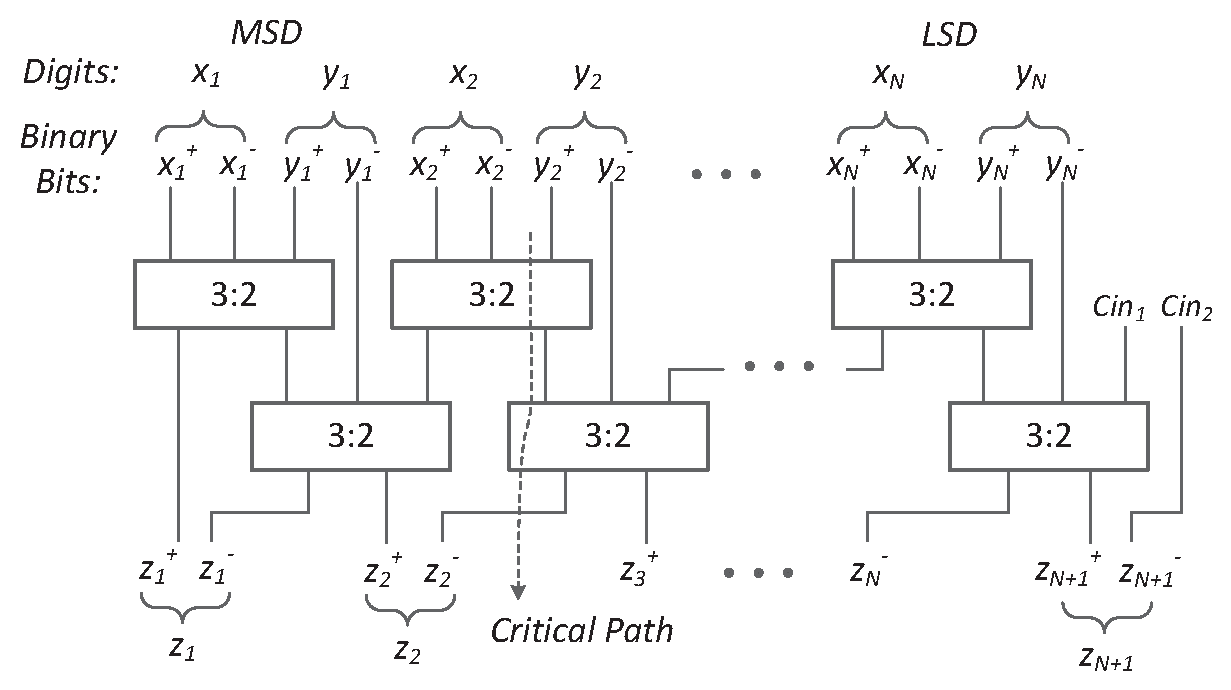
\includegraphics[width=.45\textwidth]{./figures/SDAdder.eps}
  \vspace{-1ex}
  \caption{An $N$-digit binary digit-parallel online adder. Both inputs and outputs are represented using SD representation. ``3:2'' denotes a 3:2 compressor.}
  \label{Fig:Radix2SD_adder}
  \vspace{-2ex}
\end{figure}

\subsection{Design Trade-offs for Adders}
In this section, we demonstrate the benefits of CSA and OA in accuracy and performance, as well as the area overhead in comparison to RCA. As an example, the maximum word-lengths with respect to a variety of operating frequencies for RCA, CSA and OA are illustrated in Fig.~\ref{Fig:max_wl_adder}. In this experiment, circuits are operated with timing closure, i.e. the conventional design scenario is evaluated for all structures. We consider the operand word-length of adders ranging from 32-bit to 4-bit.
%
\begin{figure}[tbp]
  \centering
  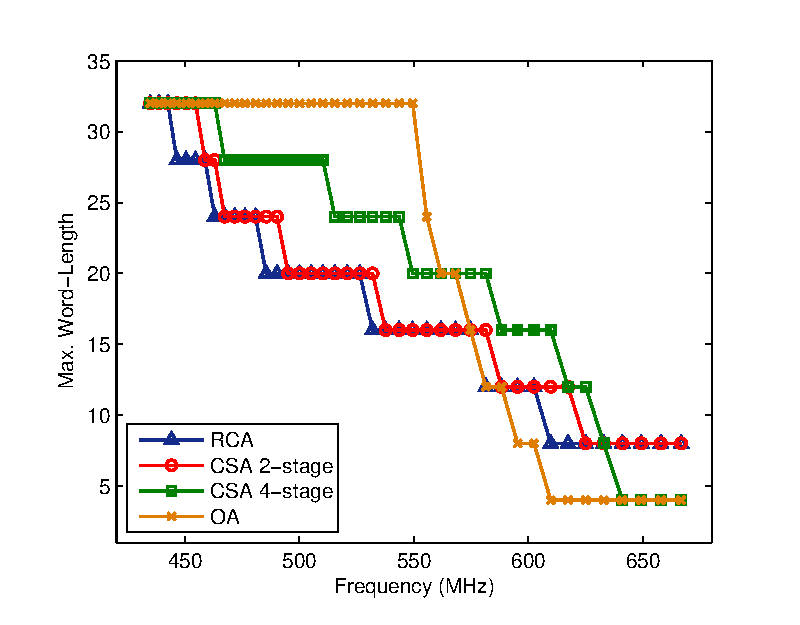
\includegraphics[width=.5\textwidth]{./figures/exp/max_wl.eps}
  \vspace{-4ex}
  \caption{The maximum word-lengths of different adder structures with respect to a variety of frequencies. The results are obtained from Xilinx ISE 14.7.}
  \label{Fig:max_wl_adder}
  \vspace{-2ex}
\end{figure}

As can be seen in Fig.~\ref{Fig:max_wl_adder}, for a relatively relaxed frequency requirement (e.g. 470 MHz), both CSA and OA can be implemented with greater word-lengths than RCA. For CSA, this is because the stage parallelism enables a larger word-length, even though the multiplexer delay limits the precision of each CSA stage in comparison to RCA. For OA, an even larger gap in word-length can be observed when compared to RCA. Additionally, unlike RCA and CSA of which the maximum word-length drops gradually with the increment of frequency, OA maintains full precision across a large range of frequencies. This is expected, because the critical path delay of OA is theoretically irrelevant to the operand word-length as discussed in Section~\ref{subsec:online_adder}. However, we also observe that given a large frequency requirement, the word-length of OA drops drastically. Besides, CSA cannot be implemented with larger precision than RCA either, because in this case the multiplexer delay becomes comparable to the delay of the carry chain for CSA, and it inhibits the benefits of parallelism.
%
\begin{figure}[tbp]
  \centering
  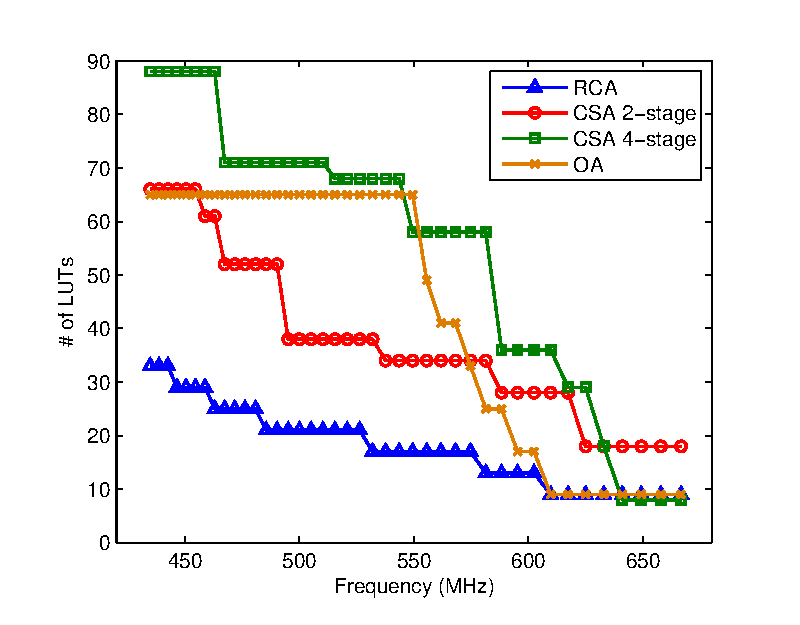
\includegraphics[width=.5\textwidth]{./figures/exp/area_adders.eps}
  \vspace{-4ex}
  \caption{The maximum area of different adder structures.}
  %\vspace{-2ex}
  \label{Fig:area_adder}
\end{figure}

We also record the corresponding area consumption of each adder structure in terms of look-up-tables (LUTs) in FPGA as depicted in Fig.~\ref{Fig:area_adder}. It can be seen that the CSA with 4 stages and 2 stages costs up to $4.5\times$ and $3.1\times$ area than RCA, respectively. OA is also up to $3.8\times$ larger than RCA. Therefore, it is necessary to provide comprehensive evaluations of different adders by considering the trade-offs between accuracy, performance and area consumption. In summary, the evaluated adder structures as well as design scenarios are summarized in Table~\ref{Table:comparison}.

\begin{table}[tbp]
\renewcommand{\arraystretch}{1.1}
\caption{Adder Structures and Design Scenarios Considered in this Paper.}
\vspace{-1.5ex}
\label{Table:comparison}
\begin{center}
\small
\begin{tabular}{c|cc}
\hline
\hline
\multirow{2}*{\textbf{Adders}} & \multicolumn{2}{c}{\textbf{Design Scenarios}} \\
& Overclocking & Traditional \\
\hline
Ripple Carry Adder & $\surd$ & $\surd$ \\
Carry Select Adder &       & $\surd$ \\
Online Arithmetic Adder  &       & $\surd$ \\
\hline
\hline
\end{tabular}
\end{center}
\vspace{-2ex}
\end{table}
\normalsize


\section{Evaluation of Optimum Adder Structure}\label{sec:optimum_adder}
Generally, our evaluation could be of interest to a circuit designer in several ways. For example, suppose the algorithm designer wish the circuit to run at a given frequency within a specific area budget, while achieving the minimum output error. Besides, for many applications, the circuit designer would wish the circuit to operate as fast as possible with the minimum resource usage, whilst a certain error budget can be tolerated. In both cases, decisions must be made on which adder structure achieves this minimum, and which design scenario should be adopted. In our experiments, the inputs are set to randomly generated data following uniform distribution.
%whether the circuit should be overclocked.

\subsection{Optimum Adder with Given Frequency and Area Requirements}\label{subsec:adder_freq_area}

For this type of applications, the available area and expected operating frequency are given at the design time. As an example slice through the design space, in Fig.~\ref{Fig:Error_Area} we record the mean relative error (MRE) with respect to a range of operating frequencies for different design scenarios, when the area budget is set to 35 LUTs and 55 LUTs separately. MRE can be calculated as given by (\ref{Eq:MRE}), where $E_{error}$ and $E_{out}$ denote the mean value of error and the mean value of correct outputs, respectively. Notice that the optimum adder design metric that achieves the minimum MRE is labeled.
%
\begin{eqnarray}\label{Eq:MRE}
  MRE=\frac{E_{error}}{E_{out}}\times100\%
\end{eqnarray}

In Fig.~\ref{subfig:error_area_lut35}, the area budget is set to 35 LUTs. For all frequency values, the overcloced RCA achieves no larger MRE than the RCA with truncated operand word-lengths. This is in accordance with the analysis in Section~\ref{subsec:rca}. We also notice that both CSA and OA cannot be implemented with full precision due to area limitation, and this leads to large truncation errors. Despite that the CSA with 4 stages is best for some frequencies, in general the overclocked RCA is the optimum design for most frequency requirements.

However if the area budget is released to 55 LUTs, OA can be implemented with original word-length. Additionally CSA can also be implemented with larger precision, but still with truncation errors. Therefore as shown in Fig.~\ref{subfig:error_area_lut55}, OA serves as the optimum design with respect to a wide range of frequency requirements. For higher frequencies, the MRE of OA increases rapidly, and CSA with 4 stages outperforms for higher frequencies. Similar to Fig.~\ref{subfig:error_area_lut35}, the overclocked RCA is the optimum design for even higher frequencies, because in this case the CSA can only be implemented with small precisions, and the multiplexer delay limits the benefits of parallelism.

\begin{figure}[tbp]
  %\vspace{-2ex}
  \centering
  \subfigure[Available LUT=35.]{
  \begin{minipage}[c]{0.5\textwidth}
    \centering
    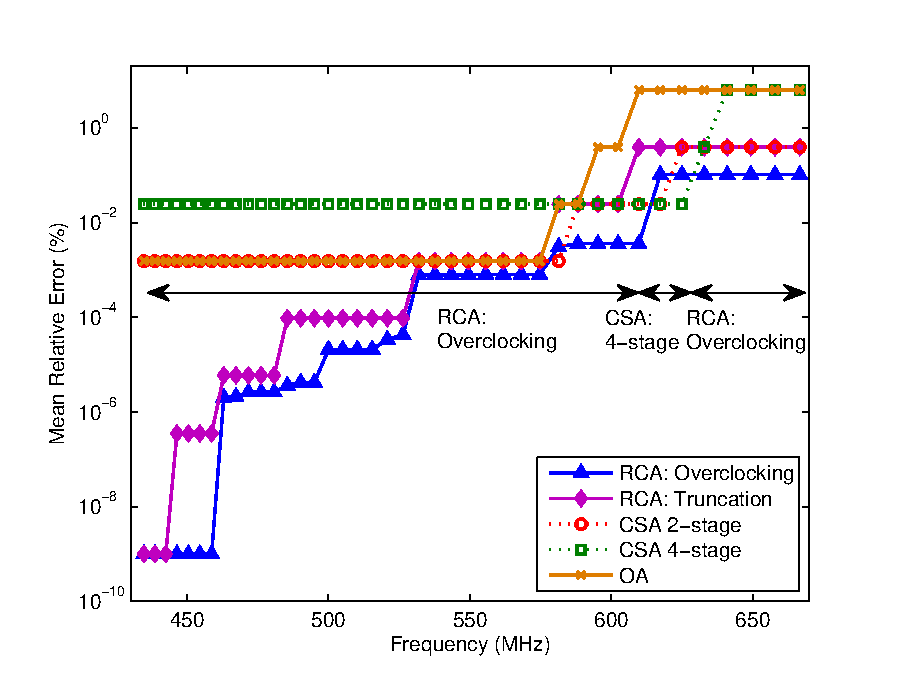
\includegraphics[width=\textwidth]{./figures/exp/Error_LUT35.eps}
    \label{subfig:error_area_lut35}
    \vspace{-2.5ex}
  \end{minipage}%
  }
  \subfigure[Available LUT=55.]{
  \begin{minipage}[c]{0.5\textwidth}
    \centering
    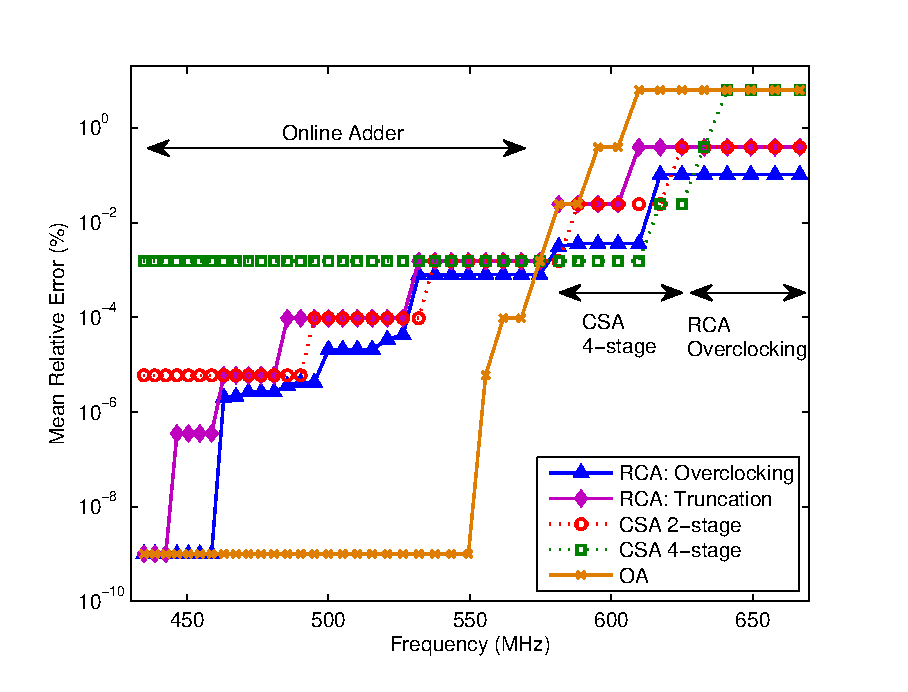
\includegraphics[width=\textwidth]{./figures/exp/Error_LUT55.eps}
    \label{subfig:error_area_lut55}
    \vspace{-2.5ex}
  \end{minipage}
  }
  \vspace{-2.5ex}
\caption{Two examples of comparisons between different design scenarios and adder implementations with limited area budget. RCA is evaluated with both overclocking and truncation scenario, whereas CSA and OA are evaluated with truncation scenario only. Design scenario with minimum error is labeled.}
\label{Fig:Error_Area}
\vspace{-2ex}
\end{figure}

The results shown in Fig.~\ref{Fig:Error_Area} can be further extended by testing with a variety of area constraints. In this case, we can map the optimum design scenarios into the design space of different operating frequencies and area consumptions, as shown in Fig.~\ref{Fig:adder_3d_FreqArea}. In general this graph can be divided into several regions. Firstly, if the frequency requirement is moderate whilst the area budget is large enough to implement an OA in full precision, it will be the optimum design. This is because long carry chains are eliminated from OA such that it can maintain full precision for a wide range of frequency values. Also this is in accordance with the results in Fig.~\ref{subfig:error_area_lut55}. Secondly, CSA is a better design choice for high frequency requirements and large area budget, because it is originally designed with high speed operation. Besides, each stage of CSA is implemented in the FPGA with fast carry logic~\cite{Virtex6}, hence it runs even faster than OA. Thirdly, for a tighter area budget only part of OA and CSA can be implemented, whereas RCA still keeps original precision. In this situation, area becomes the limitation factor. Both OA and CSA generate truncation errors, which are greater than the overclocking error of RCA. Therefore, the overclocked RCA is the optimum design option across almost the entire frequency domain. Furthermore, the precision of RCA is also limited under very stringent area constraints. This causes truncation errors for every design option. Nevertheless, RCA with either overclocking or truncation scenario equally serves to be optimal, because it maintains more precision than OA and CSA for a specific area budget.

\begin{figure*}[tbp]
  \centering
  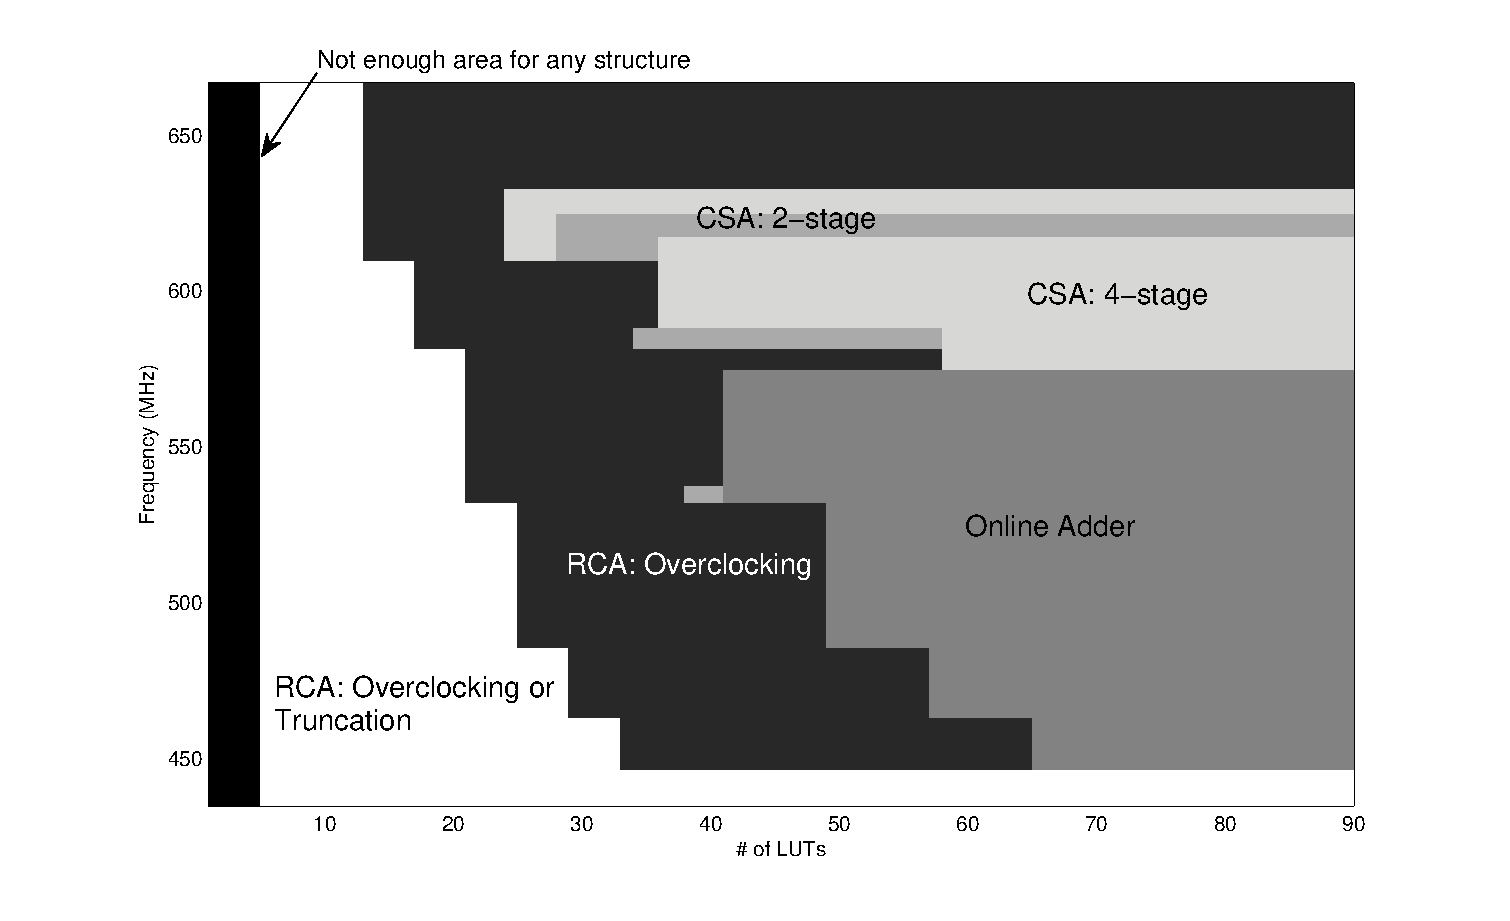
\includegraphics[width=.7\textwidth]{./figures/exp/3d_FreqArea.eps}
  \vspace{-3ex}
  \caption{Mapping of optimum design metric of adders, which achieves minimum error with respect to a variety of frequency and area constraints. The original word-length of all adders is 32-bit. The results are obtained from Xilinx ISE 14.7.}
  \label{Fig:adder_3d_FreqArea}
\end{figure*}

\subsection{Optimum Adder with Given Accuracy and Area Budgets}\label{subsec:adder_accuracy_area}
If the circuit is designed to operate as fast as possible with minimum area, whilst a certain amount of imprecision can be tolerated, the optimum adder design metric can also be determined as illustrated in Fig.~\ref{Fig:adder_3d_ErrorArea}. In this set of experiments, the error budget is evaluated in terms of MRE, which varies from $10^{-6}\%$ to $10\%$. For a given MRE, the optimum adder is selected with maximum operating frequency. In this case, if multiple designs can operate with the same frequency, the optimum design is then selected based on actual area consumption within the area constraint.
%
\begin{figure*}[tbp]
  \centering
  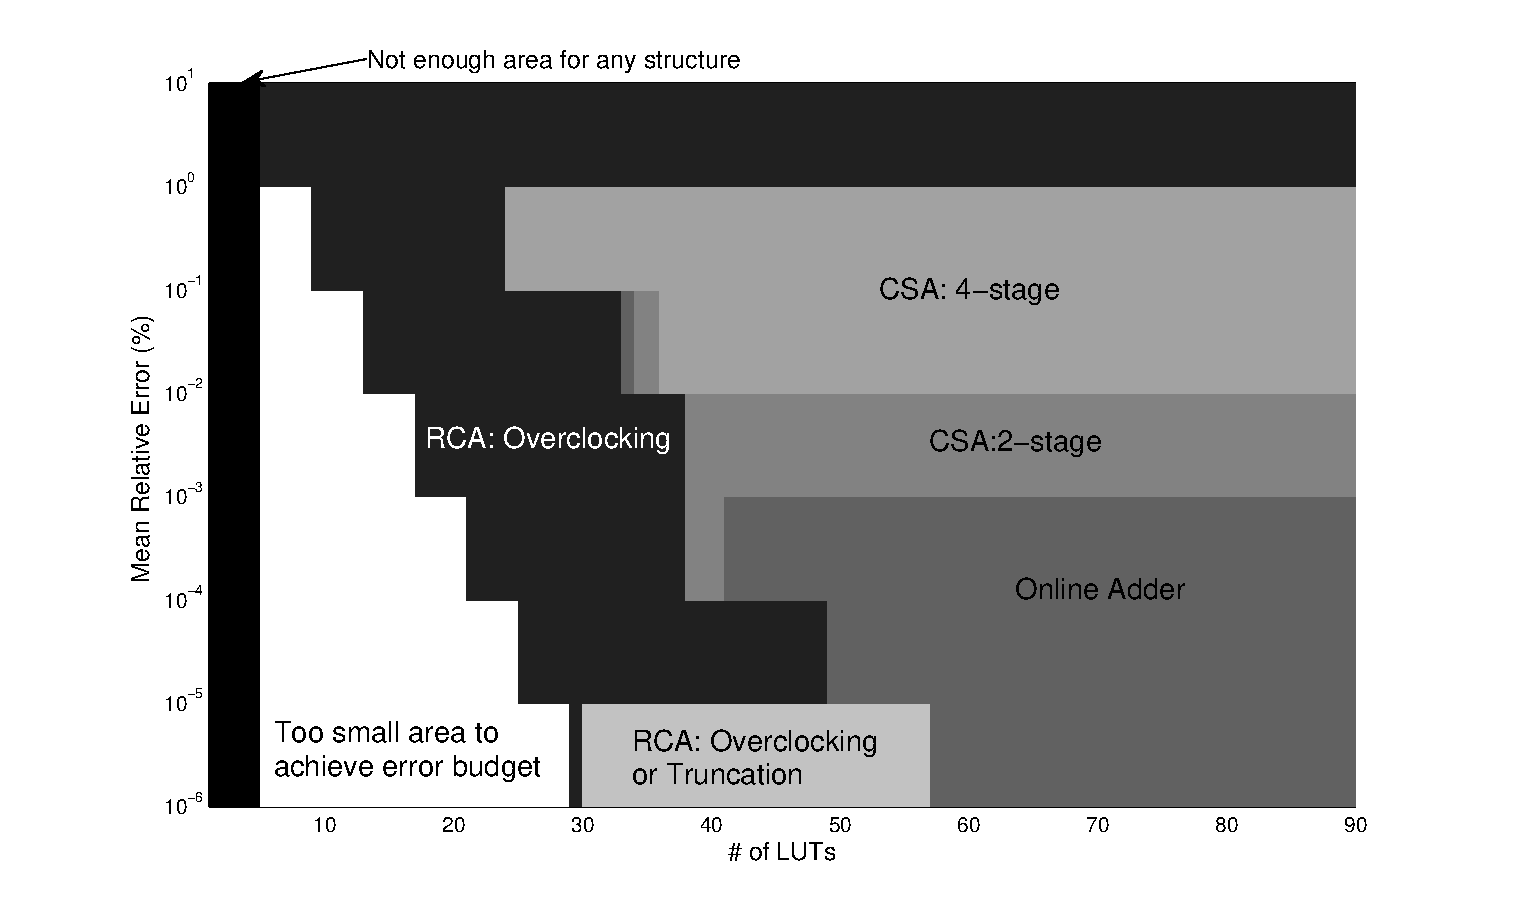
\includegraphics[width=.7\textwidth]{./figures/exp/3d_ErrorArea.eps}
  \vspace{-3ex}
  \caption{Mapping of optimum design metric of adders, which achieves highest frequency with respect to a variety of accuracy and area constraints. The original word-length of all adders is 32-bit. The results are obtained from Xilinx ISE 14.7.}
  \label{Fig:adder_3d_ErrorArea}
\end{figure*}

Similar to the analysis in Section~\ref{subsec:adder_freq_area}, for tight accuracy requirement and large area budget, OA is the optimum design choice because it keeps full precision while running at high frequencies. If relaxing the accuracy requirement (e.g. $0.01\%$), CSA gradually outperforms because its precision loss is less than that of OA. Once again, if area budget is tightened, the RCA becomes the best design choice, because the precision of OA and CSA is largely limited. Furthermore, when the accuracy requirement is released (e.g. over $1\%$), RCA can operate with the fastest frequency across most area constraints.



\section{Conclusion}\label{sec:conclusion}
In this paper, we have quantified design trade-offs for three different adder structures: ripple carry adder, carry select adder and online adder. Two design scenarios that can sacrifice accuracy for better performance have been evaluated: one is the conventional design scenario in which timing closure is achieved by truncating precision, the other is the overclocking scenario where timing violations are allowed to occur. By combining both adder structures and design scenarios, we have demonstrated experimentally the optimum design option when considering a variety of frequency-accuracy-area trade-offs. We have shown that applying the overclocking scenario to RCA can be beneficial with limited area budget, whilst applying the conventional scenario to online adder is an optimal design choice with relaxed area requirements.

In the future we wish to provide similar evaluation to other arithmetic primitives, such as multipliers. Other evaluation metrics, such as energy consumption and throughput, can also be included in the future.

% and more complex designs and applications.

%\section*{Acknowledgment}


\bibliographystyle{./IEEEtran}

\bibliography{./IEEEabrv,./Reference}


\end{document}


